\chapter{Discussion}
Discussion about the results produced by the thesis.

\section{Robustness}
It is important to know that a hypervisor can never increase robustness of a single OS, only make it more isolated from errors from another OS. Potentially, the hypervisor itself can become the source of an error causing the collective system to fail, see figure~\ref{fig:monitor}.

\begin{figure}[H]
\centering
\begin{subfigure}[b]{0.45\textwidth}
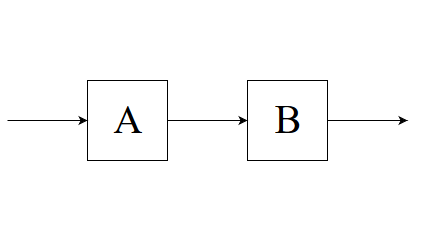
\includegraphics[width=\textwidth]{./img/discussion_nomonitor.png}
\caption{Integrity of A is dependent on integrity of B.}
\end{subfigure}
\begin{subfigure}[b]{0.45\textwidth}
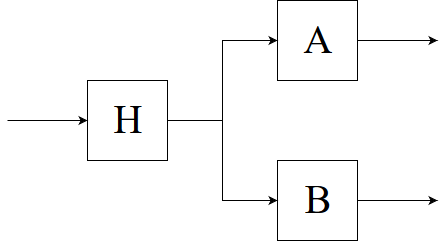
\includegraphics[width=\textwidth]{./img/discussion_monitor.png}
\caption{Integrity of A is isolated from B, but is instead dependent on H.}
\end{subfigure}
\caption{}
\label{fig:monitor}
\end{figure}

Keeping this in mind is important when discussing the robustness of a MCS.

%Adding a new link to a chain can never increase the chains strength, but hopefully the new link is strong enough to not decrease the chains strength. Much like this analogy, the robustness of a system with a hypervisor can not be as good as one without a hypervisor potentially can be. If a system only is dependant on one function to not fail, adding a new function in series can never increase robustness.

\section{Information retrieval}
%Printing to SYSLOG takes time and has an effect on the system that is being monitored.\\
The hardware timer used when measuring execution times requires very little processor time, but still some. This adds an ever so slight error to the execution times. The data was deemed to be of good enough quality anyway.

%\section{Errors}
%TODO: expand
%Unregistered exception, accessing restricted AXI bus address. Should be avoided by accessing via OS instead of address. All address space should be handled by the OS/monitor, allowing or restricting access to certain address spaces. Probably not correctly setup.

\section{Virtualization resource gain vs resource loss}
%At what point is it not worth it to have a non-critical system application on the same hardware? 
As described earlier, higher frequencies of RTOS tasks leads to more overhead. Disregarding the maximum frequency of 1~kHz for tasks in FMP, the maximum frequency for the functions in the implemented system would be just under 40 kHz, leading to an overhead of 24\% for the hypervisor. This gives the GPOS no time at all for the case when every other task executes for its WCET. However, assuming every task executes for its median execution time, the GPOS can execute for 31\% of the time at 40~kHz. This gives a very good combination of throughput for the entire system and real-time guarantees for the safety-critical tasks at the cost of a maximum overhead of 24\%. This is visualized in figure~\ref{fig:cpu_util}.

\begin{figure}[H]
\centering
\begin{subfigure}[b]{0.49\textwidth}
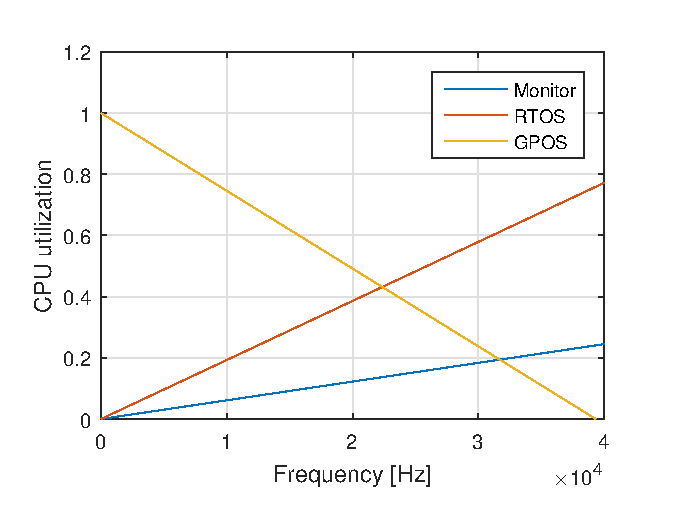
\includegraphics[width=\textwidth]{./img/discussion_util_wcet.eps}
\caption{Worst case execution time}
\end{subfigure}
\begin{subfigure}[b]{0.49\textwidth}
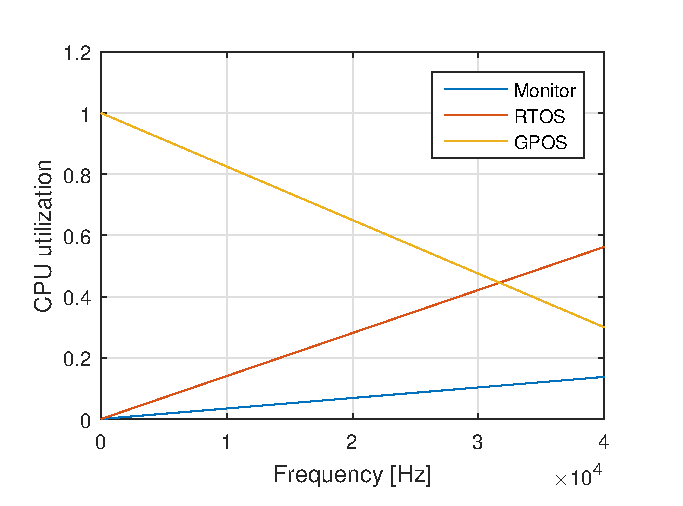
\includegraphics[width=\textwidth]{./img/discussion_util_med.eps}
\caption{Median execution time}
\end{subfigure}
\caption{CPU utilization of monitor, RTOS and GPOS. Note that for the WCET of tasks, 100\% CPU utilization by the monitor and RTOS is reached just before 40 kHz.}
\label{fig:cpu_util}
\end{figure}

%Deterministic system - work towards 100\%, anything under that: reduce clock frequency to reduce power consumption and reach 100\%.\\

%Sporadic system - probably want to be around ~50\% utilization to maintain 100\% schedulability, higher depending on requirements on performance versus requirements on efficiency.

\section{Conclusion}
In the introduction of this thesis, the following research question was presented:

\begin{itemize}
\item Is virtualization an efficient approach when trying to reconcile the conflicting requirements of partitioning for safety assurance and sharing for efficient resource usage when implementing a safety-critical control system?
\end{itemize}

After the implementation, it can be clearly seen that virtualization can be a very efficient and secure approach for reconciling the conflicting requirements of partitioning and sharing. However, finding out if it is efficient in the industry as a whole requires additional research in technical aspects as well as other aspects such as management and financial related ones. These are presented in chapter~\ref{sec:future_work}.
